\chapter{恒星光谱的分类}
\subsection{恒星光谱型}
\paragraph{哈佛分类法}
通过斯特藩-玻尔兹曼定律可以确定恒星的有效温度,根据有效温度由高到低可将恒星分为``O B A F G K M'',中间还具体细分为十级(如A0-A9),由于天文学界一开始误认为恒星也是按照这样的顺序来演化的,因此靠左的类型又称为\textbf{早型星},靠右的类型又称为\textbf{晚型星}。

\paragraph{MK光度级}
实际上是通过光谱分辨恒星的演化阶段,对应罗马字母I到V,将I型定义为超巨星,V型定义为主序星,后来又补充了VI型为亚矮星,VII型为白矮星。对于单个恒星的演化,主序、巨星、超巨星阶段的光度随半径增加(参考\ref{sec:evolution}节),而半径增加会导致恒星表面引力减弱,压强减小,从而压强增宽机制会减弱,产生的谱线宽度会较小,因此,可以通过谱线宽度来确定恒星的光度。\mbox{}\\

上述两种光谱分类结合使用可以分别确定恒星的演化阶段和温度,从而在赫罗图上可以读出对应的光度,并根据视星等进一步计算出恒星的距离,这种测距方法称为\textbf{分光视差}。

\paragraph{麦克斯韦-玻尔兹曼速率分布}
描述在热平衡系统下,具有不同速率的粒子的数量分布
\begin{equation}
  n_v dv=n\left({m\over 2\pi k T}\right)^{3/2}e^{-mv^2/2kT}4\pi v^2 dv
  \label{eq:maxwell}
\end{equation}

\paragraph{玻尔兹曼方程}
描述处于不同激发态的原子数量比
\begin{equation}
  {N_b\over N_a}={g_b e^{-E_b/kT}\over g_a e^{-E_a/kT}}={g_b\over g_a}e^{-(E_b-E_a)/kT}
  \label{eq:boltzmann}
\end{equation}

其中$g_b$为$b$能级的简并度(有多少量子态具有相同能量),$E_b$为$b$能级的能量。

\paragraph{萨哈方程}
描述不同电离态的原子数量比
\begin{equation}
  {N_{i+1}\over N_i}={2Z_{i+1}\over n_e Z_i}\left({2\pi m_e kT\over h^2}\right)^{3/2} e^{-\chi_i/kT}
  \label{eq:saha}
\end{equation}

以及等价形式:
\begin{equation}
  {N_{i+1}\over N_i}={2kTZ_{i+1}\over P_e Z_i}\left({2\pi m_e kT\over h^2}\right)^{3/2} e^{-\chi_i/kT}
\end{equation}

其中$Z_i$为电离态为$i$的离子的配分函数:
\begin{equation}
  Z={\sum_{j=1}^\infty g_j e^{-(E_j)/kT}\over e^{-(E_1)/kT}}=g_1 {N\over n_1}
\end{equation}

从公式上看,配分函数其实是总原子数与基态原子数之比乘以基态简并度,描述的是\textbf{原子可能的状态数之和}。由于电离涉及电离能,不同能级的原子需要的电离能不同,同时并不是所有原子都处于基态,因此萨哈方程中利用基态电离能,但是乘以配分函数就可以考虑不同激发态的平均电离能。

\subsection{赫罗图}
\begin{figure}[hbt]
  \centering
  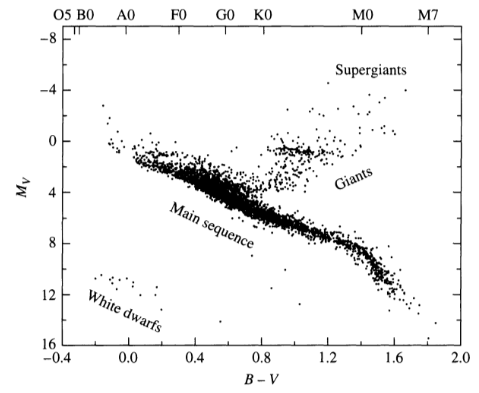
\includegraphics[width=14cm]{chapters/08/HRD}
  \caption{赫罗图}
  \label{}
\end{figure}